\section{Liv på Exoplaneter} \label{sec:liv}

Der har været mange forsøg på at definere hvad liv er, og måske findes der versioner, vi end ikke vil kunne genkende som levende. Jagten på liv andre steder fokuserer dog på, at lede efter liv som os selv, da det er svært at sige, hvad vi ellers skulle kigge efter. Men vi leder også mere generelt efter noget, der ser unaturligt ud eller ude af balance for, hvad vi ville forvente af en planet uden liv.

\subsection*{Biomarkører}

Vi kan bruge spektre til at analysere, hvilke stoffer der findes i en gas. Så hvis vi har en lyskurve fra atmosfæren på en planet (fx fundet gennem transitmetoden, mens den passerer foran en stjerne), kan vi afgøre hvilke luftarter den består af. Jordens atmosfære er meget ude af ligevægt i forhold til, hvis der ikke fandtes liv. Oxygen er eksempelvis forholdsvis reaktivt, så hvis der ikke havde liv til at producere det, ville det have bundet sig til andre stoffer - vi kender fx, hvordan jern ruster og frugt bliver brunt, hvis man lader det stå ude. Oxygen i atmosfæren ville derfor være en god indikation på, at der findes liv på en planet - en biomarkør.

På figur \ref{fig:Biospektrer} ses spektre af atmosfærerne på Jorden, Mars og Venus. Her er det tydeligt, at Jordens atmosfære adskiller sig væsentligt i form af fx mere oxygen og vand. Man hører ofte om ozonlaget, der beskytter os mod ultraviolet stråling, hvilket ses i Jordens spektrum ved linjen markeret med O$_3$. Hvis det ikke var for absorptionen ville atmosfærenens spektre følge de stiplede linjer. På alle 3 planeter ses CO$_2$ tydeligt, men Jordens spektrum er særligt domineret af absorption fra vanddamp ved både lange og korte bølgelængder.

\begin{figure}[h!]
    \centering
    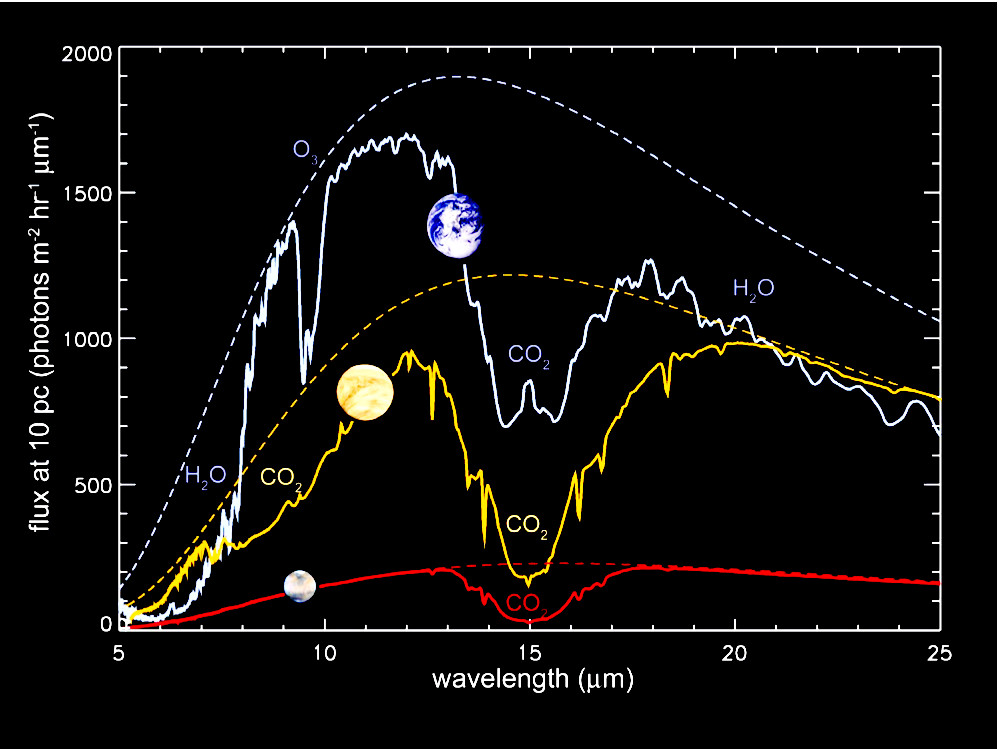
\includegraphics[width=.6\textwidth]{Astrofysik/billeder/venus-earth-mars_ir.jpg}
    \caption{Her ses spektre fra Jorden, Mars og Venus. De stiplede linjer angiver hvordan lyset ville være fordelt hvis ikke der skete absorption i atmosfæren.  \textit{Kilde: Franck Selsis and Giovanna Tinetti, Darwin proposal, 2007}} %https://light2015blogdotorg.wordpress.com/2015/03/02/searching-for-that-light-of-life/#more-756
    \label{fig:Biospektrer}
\end{figure}

\subsection*{Den Beboelige Zone}
For at finde genkendeligt liv, leder vi som sagt efter jordlignende planeter. Men hvilke krav skal vi stille til en planet, før den ligner os tilstrækkeligt?
Livet på Jorden er i høj grad baseret på kulstofforbindelser og vand. Man kunne muligvis også forestille sig liv baseret på kulstof og ammoniak eller silicium og ammoniak, men vi har aldrig fundet disse typer organismer. Livet på Jorden kan dog ikke klare sig med vand på hvilken som helst form - det kræver flydende vand. Så planeter der tillader flydende vand kan være særligt interessante.

Man har defineret et område omkring en stjerne kaldet "den beboelige zone", som ligger i den afstand fra stjernen, hvor en planet som Jorden kunne have flydende vand. Planetens atmosfære og masse har selvfølgelig betydning, men normalt vil man estimere zonen antaget en jordlignende planet. Er man for tæt på stjernen vil vandet fordampe, og er man for langt væk vil det fryse til is. Derfor er den beboelige zone tilpasset efter stjernens luminositet, så den er tæt på for små stjerner og langt væk for store stjerner. Et eksempel kan ses i figur \ref{fig:HZ}. At en planet er i den beboelige zone er dog bestemt ingen garanti for, at den er beboelig.

\begin{figure}[h!]
    \centering
    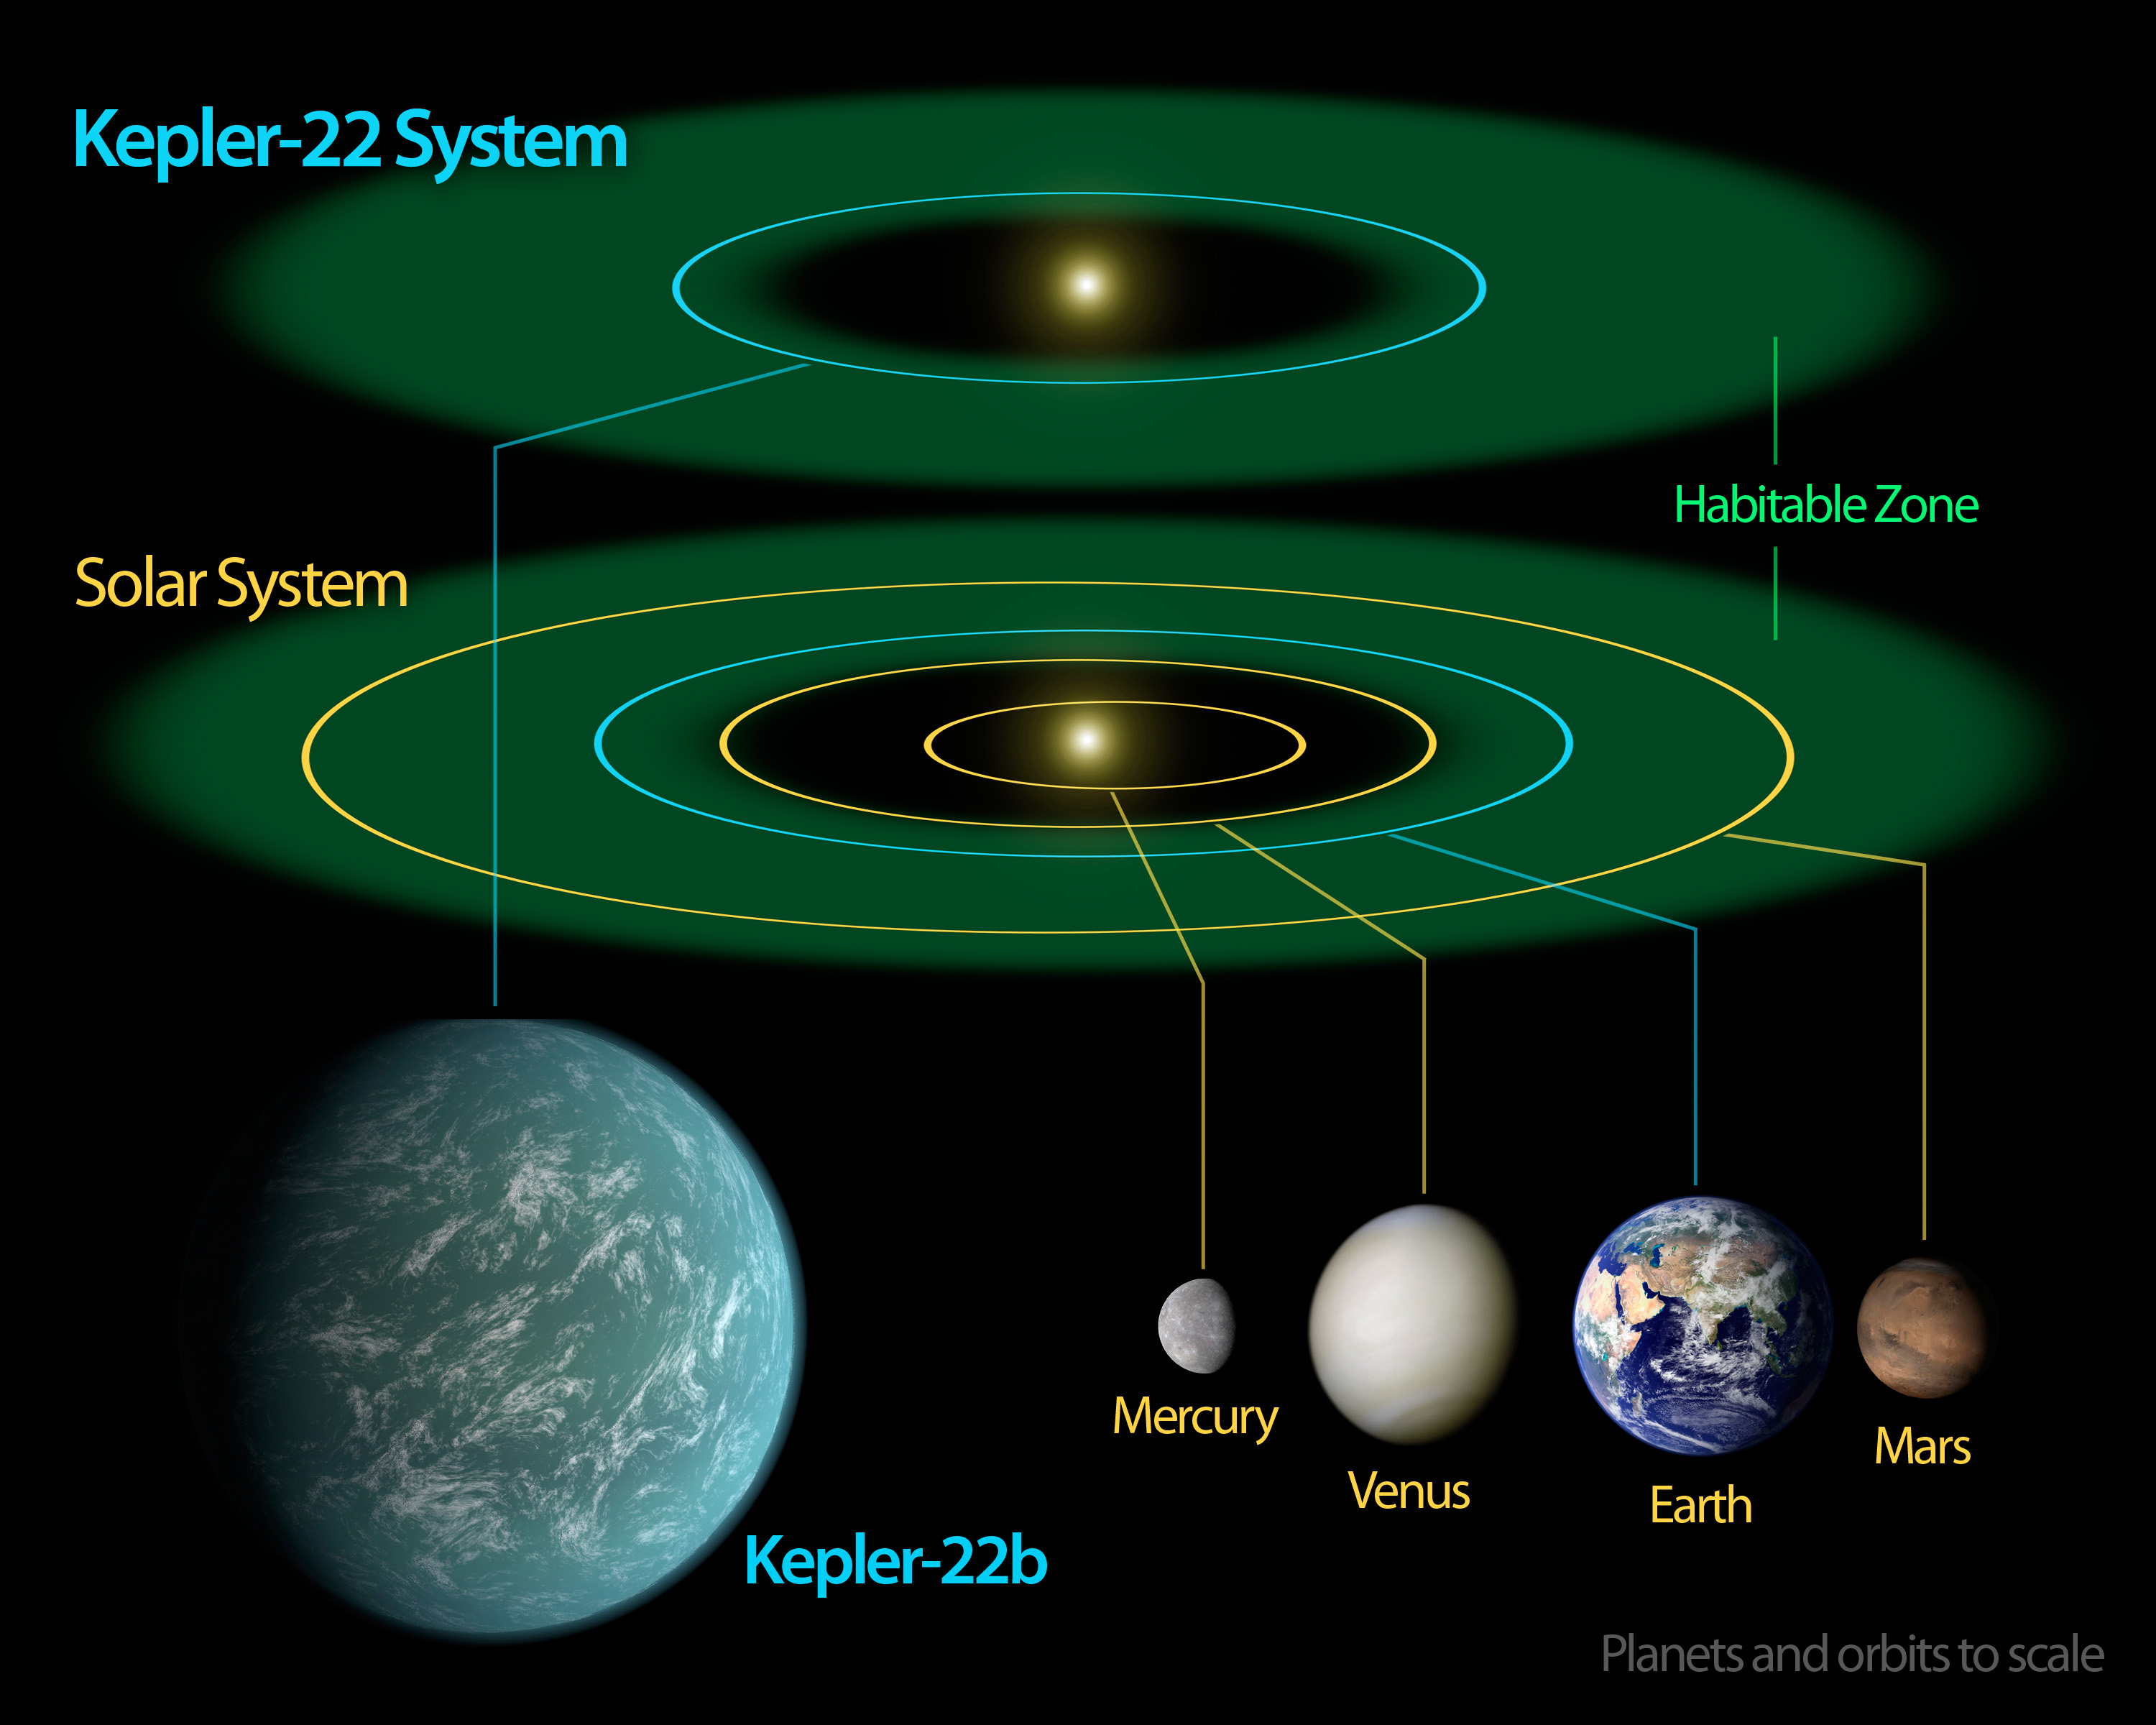
\includegraphics[width=.6\textwidth]{Astrofysik/billeder/Kepler-22_diagram.jpg}
    \caption{Illustration af et bud på den beboelige zone for Solsystemet og systemet om stjernen Kepler-22. 
    \textit{Kilde: https://commons.wikimedia.org/wiki/File:Kepler-22\_diagram.jpg}} %https://light2015blogdotorg.wordpress.com/2015/03/02/searching-for-that-light-of-life/#more-756
    \label{fig:HZ}
\end{figure}

%er den bedste taktik at lede efter en planet, der minder om Jorden, da der jo er liv her, men hvilke krav skal man stille til en såkaldt "jordlignende planet"? 
%Alt hvad vi kender til af liv på Jorden består hovedsageligt af organiske molekyler, og de interagerer på en eller anden led med molekyler som vand, ilt, kuldioxid og ammoniak. Vand er dog ikke bare vand, da liv ofte har det bedre i flyende vand, end is og vanddamp. 
Hvis man vil gå mere i dybden med om vand kan findes på den enkelte planet, kan man beregne dens overfladetemperatur, $T_p$, som
\begin{align} \label{eq:PlanetTemperatur}
    T_p = T_\star\left(\frac{1-A}{4}\right)^{1/4}\left(\frac{R_\star}{r}\right)^{1/2} \, ,
\end{align}
hvor $T_\star$ er stjernens overfladetemperatur, $R_\star$ er stjernens radius, $r$ er afstanden mellem stjernen og planeten og $A$ er planetens albedo. Albedoen er en enhedsløs konstant, der udtrykker hvor meget planeten reflekterer, da det jo kun er den energi planeten absorberer, der går til at varme den op. Denne formel bygger på en antagelse om, at der eksisterer en mekanisme, som fordeler energien på hele planetens overflade. Fx en hurtig rotationshastighed eller en atmosfære. Man kan også komme ud for at en planet er "låst" så den altid vender samme side mod Solen - i så fald vil den sandsynligvis være for varm på den ene side og for kold på den anden, men der kan være en stribe med lige den rette temperatur. Hvis der skal være flydende vand på planeten, så må $T_p$ være mellem $0$ og $\SI{100}{\degreeCelsius}$, under antagelse af nogenlunde atmosfærisk tryk. Dette illustrerer også hvor store dele af jagten på liv, der er præget af kvalificerede gæt og estimater. Hvis en planet har et tryk, der afviger meget fra \SI{1}{atm}, som vi har på Jorden, så vil temperaturintervallet, hvor vand kan eksistere i flydende form være helt anderledes eller måske ikke-eksisterende. Det er også en gråzone, hvis overfladetemperaturen jævnligt falder uden for intervallet. Det kunne fx ske hvis planetens bane er meget elliptisk, eller planeten blot er meget tæt på kanten af den beboelige zone. Det er derfor svært at sætte hårde krav til en planets afstand til sin stjerne. \\
Et andet problem med ligning \eqref{eq:PlanetTemperatur} er, at den bygger på, at planeten er i termodynamisk ligevægt, hvor den opvarmes af sin stjerne og nedkøles ved varmestråling. I Solsystemet findes der flere eksempler på, at der også er andre mekanismer i spil - fx overskydende varme i planetens indre og atmosfærer der holder på varmen. %Hvis en jordlignende planet befinder sig sådan ift. dens stjerne, at der kan eksistere flydende vand på overfladen af den, så siges planten at befinde sig i \emph{den beboelige zone}. 
\\

%Langt hen ad vejen er rummet et fantastisk vakuum, som man ikke umiddelbart skulle tænke som værende "farligt". Det er dog sådan at stjerner udsender en helt masse stråling, som er nødvendigt for eksempelvis at varme planeterne op til den nødvendige temperatur.
Selv hvis en stjernes lys er passende for flydende vand, er der andre krav for om liv også kan eksistere ved stjernen. Store stjerner lever kortere, og derved har livet formentlig ikke tid nok til at udvikles til avancerede former. Små stjerner er til gengæld meget aktive og har kraftige solvinde af partikler, der slynges ud mod planeterne. Disse består af ladede partikler med høj energi, der i værste fald kan blæse atmosfæren af en planet, hvis den ikke har et magnetfelt til at beskytte sig (og strålingen kan i sig selv være skadelig for liv at blive udsat for). Samtidig er den beboelige zone tæt på stjernen, hvis den er lille, så planeten ville blive påvirket endnu mere af solvindene. \\
%Jo højere energi strålingen har, desto mere destruktivt er det. Det kan ionisere og endda spalte ellers stabile molekyler. 
%Derudover er der også solvinde, som er en strøm af ladede partikler med ekstremt høj energi. Disse ladede partikler kan være elektroner, protoner eller heliumkerner og minder derfor om radioaktiv stråling. Forskellen er her at der er mange flere af dem og at de har ekstremt meget energi. Det der redder os på Jorden fra disse fænomener er Jordens magnetfelt og atmosfære. Uden disse ville vi ikke kunne overleve, da cellerne i kroppen ikke ville kunne klare det konstante strålingsbombardement - i stedet nøjes vi med at blive solbrændte. Derfor må det også kræves at en exoplanet kan opretholde en stabil atmosfære og gerne have et beskyttende magnetfelt. For at dette magnetfelt kan eksisterer må planeten på en eller anden led være opbygget af noget materiale, der er magnetisk i den tilstand det befinder sig i. \\

Planetens masse er også afgørende for om der kan eksistere liv, da tyngdekraften på overfladen af planeten hænger direkte sammen med massen. Hvis tyngdekraften er lidt svagere end på Jorden, kan man forvente højere organismer end her, og hvis tyngdekraften er stærkere vil det betale sig at være mere kompakt. Dette skyldes at en levende organisme skal være stabil, og jo stærkere tyngdekraften er, desto stærkere skal organismen også være, for at opretholde samme højde. Dette kan man forestille sig ved at tænke på, hvordan det føles at benytte en elevator. Når elevatoren accelereres opad presses man ned i gulvet, og når den så bremser ned igen, opnår man i kort tid en følelse af at være "lettere", hvilket blev vist teoretisk for et pendul i afsnit \ref{sec:elevator}. Denne analogi er helt valid, da en af byggestenene for den generelle relativitetsteori er Einsteins ækvivalensprincip, der kan formuleres som følgende:
\begin{center}
    \textit{Intet lokalt eksperiment kan skelne konstant acceleration og gravitation fra hinanden.}
\end{center}
Dette betyder, at i eksemplet med elevatoren er det umuligt at finde ud af om elevatoren står stille i et stærkere tyngdefelt, eller om den accelereres måske endda uden påvirkning af et tyngdefelt. \\
Der er en nedre grænse for, hvor lav planetens masse kan være, da den skal være stor nok til at kunne holde på en atmosfære - ellers vil den langsomt kunne fordampe væk. Mars lille størrelse er en af faktorerne, der har gjort, at den mistede sin. %Jordens atmosfære består af relativt små molekyler på gasform, hvorfor tyngdekraften skal have en vis styrke for at holde fast i disse. 
Er planeten for lille til at opretholde en atmosfære, vil der ikke være noget til at beskytte levende organismer og holde trykket for det flydende vand, hvilket vil gøre det umuligt, for det meste liv vi kender på Jorden at overleve. \\

Kobles massen sammen med radius til en densitet, kan vi også sætte begrænsninger på, hvad planeten kan bestå af, og det har betydning for hvilket liv der kan være. Jordens liv vil fx ikke have det særlig godt på en gasplanet. Hvis en planet er meget let, kan man godt konkludere at den må indeholde hydrogen, da intet andet ville kunne give så lav densitet. Der er også densiteter man vil forbinde med planeter af vand eller klippe. Hvis densiteten er meget høj må planeten også indeholde en vis mængde jern. \\
En anden metode til at undersøge en planets materiale er spektroskopi, som beskrevet i afsnit \ref{sec:spektrer} under spektrer. Ved at analysere spektret af en planet, kan man afgøre hvad den må bestå af.\\

%blev det beskrevet, hvordan stjerners sammensætning kan identificeres ud fra hvilke absorbtionslinjer, der observeres. Passerer lys igennem planetens atmosfære, vil der ske præcis det samme, som når lyset rejser igennem stjernen - atomerne og molekylerne interagerer med lyset. Molekyler interaktion med lys er en smule mere kompliceret end atomers interaktion, men det vigtige er at det er muligt at identificere molekyler ud fra deres spektre.\footnote{Forskellige typer spektre er essentielt i specielt mange dele af kemien, da forskellige præparater kan undersøges meget præcist. Det bruges eksempelvis i forbindelse kemisk syntese til at undersøge hvorvidt man faktisk har fremstillet det molekyle, man var interesseret i.} Hvis det er muligt at finde ud af hvordan spektret ville have set ud, hvis planeten ikke havde været der, så kan man identificere de absorbtionslinjer, der skyldes planetens atmosfære. Har man absorbtionslinjerne, kan man så identificere hvilke atomer og molekyler, disse stammer fra, selvom det nu er en del lettere sagt end gjort. Det bemærkes dog at denne metode til at bestemme atmosfæresammensætning, er afhængig af lys fra en kendt lyskilde passerer igennem planetens atmosfære. Derfor er det ikke muligt, hvis planeten kun kan "ses" med eksempelvis radialhastighedsmetoden, da det nødvendige lys ikke er tilgængeligt. \\

Er det så muligt at finde liv andre steder end på Jorden, eller er det hele blot en jagt på en ikkeeksisterende nål i en høstak af astronomisk størrelse? Det korte svar er, at det ikke er til at vide. Det kan være, at det venter lige om hjørnet, og at en af de kommende missioner til Mars finder rester af liv der. Det kan også være, at man kan lede til tid og evighed uden nogensinde at finde noget. Men ved at lede, kan vi i hvert fald sætte grænser for hvor almindeligt liv er, og hvor specielle forhold vi har. Mange forskere mener, at vi sandsynligvis vil finde liv inden for 10 år, hvis det eksisterer, i forbindelse med projekter der leder endnu grundigere end nu.
%Det er dog usandsynligt at svaret ligger gemt i en ligning, som i filmen \textit{Interstellar}. 
Jagten på liv er utroligt kompleks og fascinerende, hvilket forhåbentlig er illustreret i dette kapitel, men én ting er sikkert: Hvis man ikke leder efter nålen, så finder man den i hvert fald ikke.